\input{../../../../.preambles/02-lab_work}
\newgeometry{top=1.5cm, bottom=1.5cm, left=1cm, right=1cm}
\begin{document}
    \begin{table}[h!]
        \center
        \begin{tabular}{|C{.5}|C{.2}|C{.25}|}
            \hline
            \multicolumn{1}{|c|}{\multirow{4}{*}{Лабораторная работа № 1}} &
            Студент, группа & {{ student }}, Ф-369 \\ \cline{2-3}
            & Дата выполнения &  \\ \cline{2-3}
            & Подпись &  \\ \cline{2-3}
            Определение температуры катода и & Дата отчёта & \\ \cline{2-3}
            работы выхода материала катода & Оценка &  \\ \cline{2-3}
            & Подпись &  \\ \hline
        \end{tabular}
    \end{table}

    \emph{Цель работы:} изучение явления термоэлектронной эмиссии. Нахождение с
    помощью закона Ричардсона-Дэшмана температуры катода и работы выхода
    материала катода.
    
    \begin{figure}[h]
        \center
        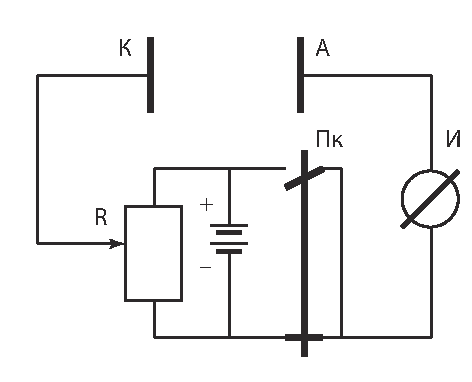
\includegraphics[width=.45\textwidth]{scheme} \hspace*{2em}
        \includegraphics[width=.35\textwidth]{appearance} \\
        \parbox{.45\textwidth}{\caption{Схема установки}} \hspace*{2em}
        \parbox{.35\textwidth}{\caption{Внешний вид установки}}
    \end{figure} 
    \begin{table}[ht]
        \center
        \caption{Определение температуры катода}
        \begin{tabular}{|C{0.06}|*{10}{C{.04}|}|*{2}{C{0.06}|}} \hline
            \( I_\textit{А} \),~мкА & 0 & 2 & 8 & 10 & 12 & 14 & 18 &
            20 & 22 & 24 & \multirow{2}{*}{\( U_\textit{н} \), В} &
            \multirow{2}{*}{\( T \),~К} \\ \cline{1-11}
            \( \ln(I_\textit{А}) \) & --- & 0,69 & 2,08 & 2,30 & 2,48 & 2,64 &
            2,89 & 3,00 & 3,09 & 3,18 & & \\ \hline
            \multirow{6}{*}{\( U_\textit{А} \),~В}
            & 2,781 & 2,000 & 1,075 & 0,868 & 0,720 & 0,575 & 0,443 & 0,220 &
            0,116 & 0,042 & 14,4 & 8169 \\ \cline{2-13}
            & 2,823 & 2,070 & 1,145 & 0,964 & 0,797 & 0,654 & 0,394 & 0,291 &
            0,188 & 0,100 & 14,8 & 7945 \\ \cline{2-13}
            & 3,000 & 2,160 & 1,219 & 1,016 & 0,857 & 0,704 & 0,456 & 0,337 &
            0,243 & 0,147 & 15,2 & 8227 \\ \cline{2-13}
            & 3,110 & 2,230 & 1,290 & 1,088 & 0,918 & 0,775 & 0,517 & 0,394 &
            0,296 & 0,197 & 15,6 & 8227 \\ \cline{2-13}
            & 3,154 & 2,285 & 1,358 & 1,159 & 0,995 & 0,837 & 0,570 & 0,452 &
            0,355 & 0,253 & 16,0 & 8169 \\ \cline{2-13}
            & 3,240 & 2,400 & 1,430 & 1,230 & 1,045 & 0,903 & 0,632 & 0,508 &
            0,413 & 0,314 & 16,4 & 8406 \\ \hline
        \end{tabular}
    \end{table}

    \begin{table}[h!]
        \center
        \caption{Определение работы выхода}
        \begin{tabular}{|*{6}{C{0.12}|}}\hline
            \( T \),~К & 8169 & 7945 & 8227 & 8169 & 8406 \\ \hline
            \( I_\textit{А} \),~мкА & 24 & 25 & 26 & 28 & 30 \\ \hline
            \( \ln(I_\textit{А}) \) & 3,18 & 3,22 & 3,26 & 3,33 & 3,40 \\\hline
            \( T^{-1}, 10^{-4}~\text{К}^{-1} \) & 1,2241 & 1,2587 & 1,2155 &
            1,2241 & 1,1896 \\ \hline
            \( W_A \),~эВ & \multicolumn{5}{c|}{2,71} \\ \hline
        \end{tabular}
    \end{table}

    \pagebreak

    \begin{figure}[h!]
        \center
        \includegraphics[width=.45\textwidth]{VAC} \hspace*{2em}
        \includegraphics[width=.45\textwidth]{WA} \\
        \parbox{.45\textwidth}{\caption{Вольт-амперные характеристики при
        различных напряжениях накала}} \hspace*{2em}
        \parbox{.45\textwidth}{\caption{К определению работы выхода}}
    \end{figure}

    \emph{Вывод:} в ходе лабораторной работы было изучено явление
    термоэлектронной эмиссии. По экспериментальным данным были рассчитаны
    температура катода при различных напряжениях накала и работа выхода катода.
\end{document}
